\documentclass{my_cv}
\usepackage{tikz}
\usepackage{multicol}
\usepackage[document]{ragged2e}
\usepackage{wrapfig}
\usepackage{graphicx}


\begin{document}
	
	
	
	\name{Gabriel E. L. Machado}
	\compInfo{Gabriel Eduardo de Lima Machado}{Engenheiro Eletricista}{23 anos}{brasileiro}
	\compInfo{Teodoro Garcia 1955}{Buenos Aires}{Argentina}{} \hfill \smash{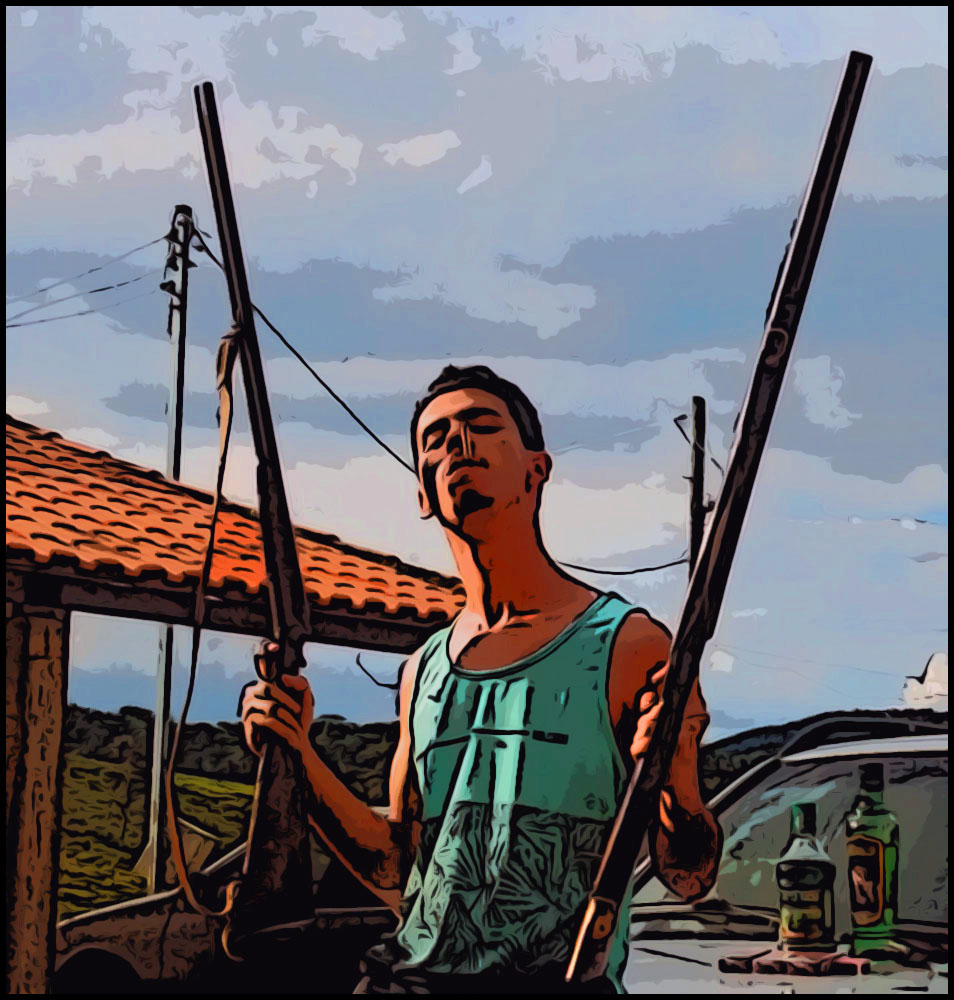
\includegraphics[width=3cm]{./foto.jpg}}
	
	\begin{multicols}{2}
		
	\contact{+55 32 9 8489 8654}
	{gabriel.machado@engenharia.ufjf.br}
	{www.linkedin.com/in/gabriel-e-l-machado}
	{https://github.com/GDX64}
		
	\section{Formação}
	\justify
	\datedsubsection{Escola Técnica Pandiá Calógeras (ETPC)}{2011--2013}
	Cursei o ensino médio e técnico em eletromecânica na ETPC em Volta Redonda.
	
	\datedsubsection{Universidade Federal de  Juiz de Fora (UFJF)}{2014--2019} 
	Atualmente sou aluno do curso de engenharia elétrica com ênfase em eletrônica na UFJF, com previsão de formatura em dezembro de 2019. Este curso conta com uma grade contendo o básico da engenharia elétrica, e matérias mais específicas de processamento de sinais, redes e eletrônica.
	
	\datedsubsection{Universidade de Buenos Aires (UBA)}{2019}
	Estou em um intercâmbio com a UBA desde fevereiro de 2019 cursando matérias do nível graduação/maestria que não estão presentes no curso da UFJF: processamento de fala, filtros adaptativos, processamento de imagens, processamento de sinais biomédicos e conteúdos relacionados a machine learning.
	
	\section{experiências laborais}
	\datedsubsection{AG Plast - Juiz de Fora}{2018}
	Realizei um estágio de 180h na empresa AG Plast em Juiz de Fora onde trabalhei com planilhas de dados de produção e relatórios de manutenção.
	
	\datedsubsection{PSA - Palomar, Argentina}{2019}
	Realizei um estágio de 240h na planta PSA (Peugeot Citroën) na província de Buenos Aires, cidade de Palomar, onde participei da elaboração de planos de manutenção e estoque de reposição de peças.
	
	\datedsubsection{UFJF - Juiz de Fora}{2014--2017}
	Dentro da própria faculdade fui monitor de física por três anos (2015-2017), auxiliando na elaboração e aplicação de exames e consultoria de alunos. Participei da equipe de robótica RINOBOT na parte de controle, comunicação (com protocolos  xbee, TCP, Bluetooth) e programação de microntroladores (esp-8266, esp-32, ATMega 16).
	
	\section{Línguas}
	\centering
	\begin{tabular}{c|c|c}
	Português & Inglês & Espanhol \\
	nativo   & avançado& avançado \\
	\end{tabular}
	\vspace{0.5cm}
	\justify
	Experiência desenvolvimento de conversação e leitura de textos técnicos e do cotidiano nas línguas estrangeiras citadas.

	\section{softwares}
	\begin{itemize}
		
	\item Conhecimentos em softwares de simulação e desenho de circuitos elétricos: Tina  TI, LT Spice, PSIM, Proteus, etc.
	\item Conhecimento em softwares de edição de imagem, texto e desenhos vetoriais: Inkscape, Photoshop, Latex, Microsoft Word.
	\item Programas de cálculo e manipulação de dados: Excel, biblioteca Pandas da linguagem Python e Matlab.
	\item Sistemas operacionais: Linux, com experiência em linha de comando e acessos remotos à servidores; Windows.
	
	\end{itemize}

	\section{Programação}
	\justify
	Durante a jornada acadêmica pude desenvolver boa habilidade para interpretar problemas e solucioná-los através de código em trabalhos de circuitos eletrônicos; internet das coisas; simulação física; sistemas de controle; processamento de imagens, fala, sinais biomédicos e sistemas gráficos em modelos tridimensionais. Obtive também experiência com diversas linguagens de programação, aprendendo a escolher a mais adequada para cada situação. 
	
	\subsection{linguagens}
	\begin{itemize}
		\item Avançado: Matlab, C, Python.
		\item Intermediário: C++, VB, JS.
		\item Básico: Verilog, Julia, Bash/Shell.
	\end{itemize}

\end{multicols}	
\end{document} ​